\subsection{Sprint 6}

\subsubsection{Introduction}
During sprint 6 the team focused on refactoring the script with the latest architecture, and refactor socket for screen, and finishing the US related to the pacman game. 

\subsubsection{Spikes}

\begin{itemize}
    \item Refactor script update with latests architecture: \href{https://tree.taiga.io/project/joseluis-teran-coffeetime/us/215?milestone=396824}{US id-215}
    \item Refactor socket client for screen bassed on latest architecture: \href{https://tree.taiga.io/project/joseluis-teran-coffeetime/us/216?milestone=397461}{US id-216}
\end{itemize}

\subsubsection{POCs}

No proofs of concept (POCs) were conducted in this sprint.

\subsubsection{Technical Justification}
In Sprint 6 the decision was made to refactor the script update and priorize US of pacman. The decision was made based on the following:

\begin{itemize}
    \item  Being able to execute the game. 
    \item  Terminate the US of pacman that were in carry over in order to finish pacman game.
\end{itemize}

\newpage

\PassOptionsToPackage{unicode}{hyperref}
\PassOptionsToPackage{hyphens}{url}
\documentclass{article}
\setcounter{secnumdepth}{6}

\usepackage{amsmath,amssymb}
\usepackage{lmodern}
\usepackage{iftex}
\usepackage[letterpaper, margin=1in, top=0.5in, bottom=1in]{geometry}
\usepackage{listings}
\usepackage{color}
\usepackage{titling}
\usepackage{graphicx}
\usepackage{hyperref}

\ifPDFTeX
  \usepackage[T1]{fontenc}
  \usepackage[utf8]{inputenc}
  \usepackage{textcomp} 
\else 
  \usepackage{unicode-math}
  \defaultfontfeatures{Scale=MatchLowercase}
  \defaultfontfeatures[\rmfamily]{Ligatures=TeX,Scale=1}
\fi
\IfFileExists{upquote.sty}{\usepackage{upquote}}{}
\IfFileExists{microtype.sty}{
  \usepackage[]{microtype}
  \UseMicrotypeSet[protrusion]{basicmath} 
}{}
\makeatletter
\@ifundefined{KOMAClassName}{
  \IfFileExists{parskip.sty}{
    \usepackage{parskip}
  }{
    \setlength{\parindent}{0pt}
    \setlength{\parskip}{6pt plus 2pt 2pt}}
}{
  \KOMAoptions{parskip=half}}
\makeatother
\usepackage{xcolor}
\usepackage{graphicx}

\makeatletter
\def\maxwidth{\ifdim\Gin@nat@width>\linewidth\linewidth\else\Gin@nat@width\fi}
\def\maxheight{\ifdim\Gin@nat@height>\textheight\textheight\else\Gin@nat@height\fi}
\makeatother
\setkeys{Gin}{width=\maxwidth,height=\maxheight,keepaspectratio}
\makeatletter
\def\fps@figure{htbp}
\makeatother
\setlength{\emergencystretch}{3em} 
\providecommand{\tightlist}{
  \setlength{\itemsep}{0pt}\setlength{\parskip}{0pt}}

\ifLuaTeX
  \usepackage{selnolig}  
\fi
\IfFileExists{bookmark.sty}{\usepackage{bookmark}}{\usepackage{hyperref}}
\IfFileExists{xurl.sty}{\usepackage{xurl}}{} 
\urlstyle{same}
\hypersetup{
  hidelinks,
  pdfcreator={LaTeX via pandoc}}

\title{Artifacts - Sprint 6}
\date{}

\begin{document}

\maketitle

\hypertarget{sos-s3} {
\section{Scrum of Scrums}\label{Scrum of Scrums} 
At that time, the team had reorganized to move forward on console, bridge and game Epics.
Mainly the architecture for running the game.jar scripts was updated, client socket communication plus bridge screen communication was implemented, and the functional US of the Pacman game was finalized. Then, in the Lead's Daily a brainstorming session was held to agree on a refactoring of Pacman with the update of the new bridge.jar and also the refactoring of the last script related to the architecture and it was concluded to move forward with the remaining US on the weekend to finish the sprint with half of the estimated points.
}

\href{https://github.com/Pending-Name-21/pac-man/pull/10}{Link: Pacman-Refactor - Pull Request on GitHub}.

\href{https://github.com/Pending-Name-21/miscellany/pull/17}{Link: Refactor-Script - Pull Request on GitHub}.

\href{https://tree.taiga.io/project/joseluis-teran-coffeetime/taskboard/sprint-6-3003}{Link: User Stories of Sprint 6 on Taiga}.

\begin{figure}
\centering
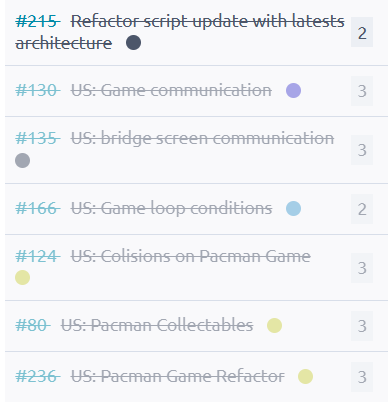
\includegraphics[width=16cm, height=10cm]{./assets/US-Sprint6.png}
\end{figure}

\hypertarget{burndownchart-s3}{
\section{Burn Down Chart}\label{Burn Down Chart S3}}
\href{https://tree.taiga.io/project/joseluis-teran-coffeetime/taskboard/sprint-6-3003}{Link: Sprint 6 Board on Taiga}.

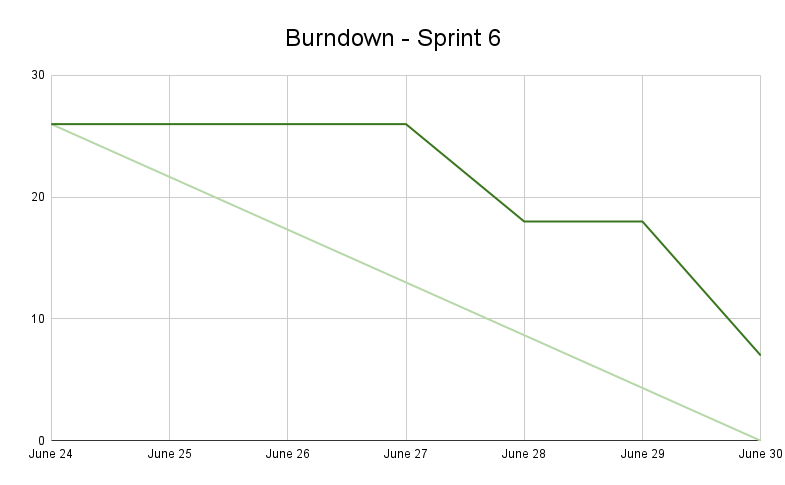
\includegraphics[width=\textwidth]{./assets/Burndown-Sprint6.png}

\hypertarget{startstopcontinueactionitems-s3}{
\section{Start-Stop-Continue-Action Items}\label{Start-Stop-Continue-Action Items S6}}
\href{https://miro.com/app/board/uXjVKDO7l8M=/?moveToWidget=3458764591631763576&cot=14}{Link: Start-Stop-Continue-Action Items Sprint 6 on Miro}.

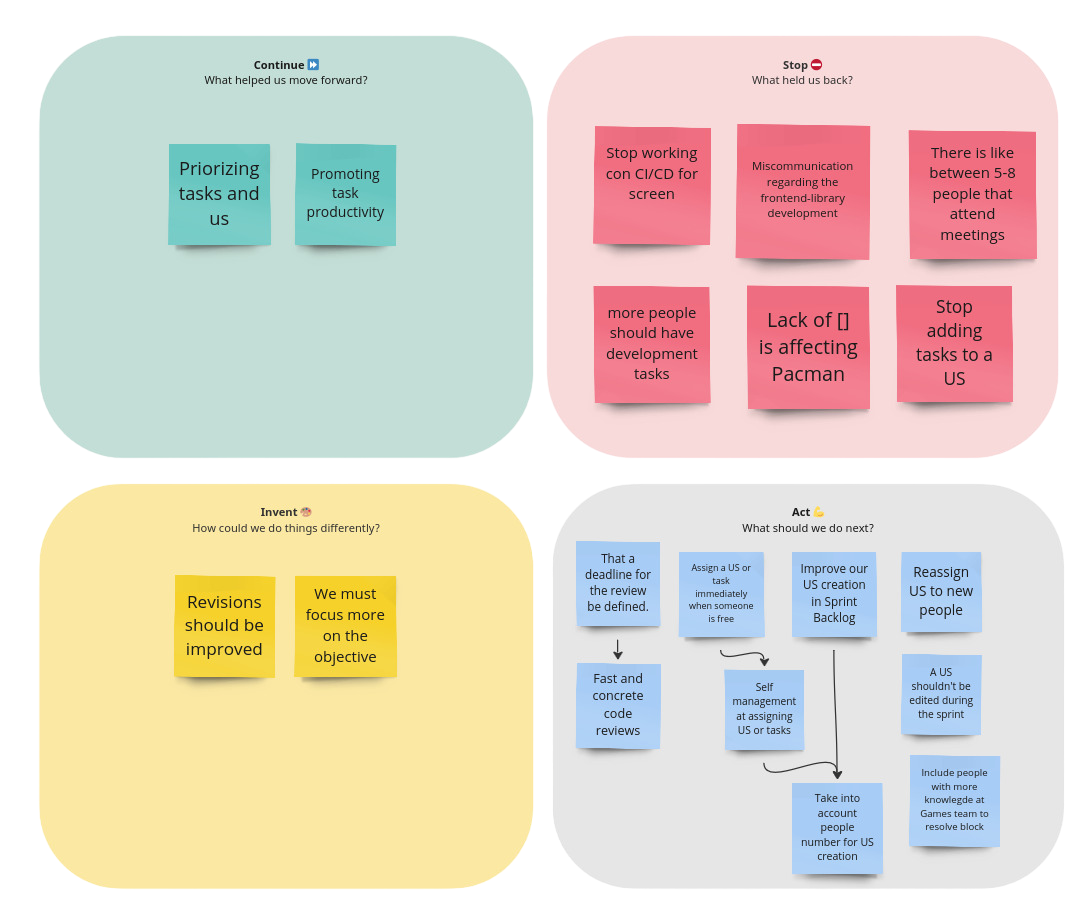
\includegraphics[width=\textwidth]{./assets/retrospective-s6.png}

\end{document}

\documentclass{article}
\usepackage{hyperref}
\usepackage{parskip}

\begin{document}

    \title{Backlog - Sprint 6}
    \author{}
    \date{}
    \maketitle

    \section*{Task Board}
    \href{https://tree.taiga.io/project/joseluis-teran-coffeetime/taskboard/sprint-6-3003}{Sprint 6 Task Board}

    \section*{Completed User Stories}

    \begin{enumerate}
        \item \textbf{Refactor script update with latests architecture} \\
        \textit{Assigned to:} Victor Villca \\
        \textit{Status:} Done in Sprint \\
        \textit{Component:} CONSOLE
        \item \textbf{Game Communication} \\
        \textit{Assigned to:} Jose Prado, Axel Javier \\
        \textit{Status:} Done in Sprint \\
        \textit{Component:} SCREEN
        \item \textbf{Bridge Screen Communication} \\
        \textit{Assigned to:} Santiago Concha, Luiggy Mamani, Alex Paca \\
        \textit{Status:} Done in Sprint \\
        \textit{Component:} CONSOLE
        \item \textbf{Game Loop Conditions} \\
        \textit{Assigned to:} Santiago Concha, Alex Paca, Emanuel Galindo, Jhael Arce, Fabian Romero \\
        \textit{Status:} Done in Sprint \\
        \textit{Component:} BRIDGE
        \item \textbf{Colisions on Pacman Game} \\
        \textit{Assigned to:} Victor Villca, Ronaldo Mendoza  \\
        \textit{Status:} Done in Sprint \\
        \textit{Component:} PACMAN GAME
        \item \textbf{Pacman Collectables} \\
        \textit{Assigned to:} Josue Prado \\
        \textit{Status:} Done in Sprint \\
        \textit{Component:} PACMAN GAME
        \item \textbf{Pacman Game Refactor } \\
        \textit{Assigned to:} Victor Villca \\
        \textit{Status:} Done in Sprint \\
    \end{enumerate}

    \section*{Carryover User Stories}

    \begin{enumerate}
        \item \textbf{Tic Tac Game Implementation} \\
        \textit{Assigned to:} Axel Javier, Luiggy Mamani, Emanuel Galindo, Jose Luis \\
        \textit{Status:} Carryover \\
        \textit{Component:} TIC-TAC
        \item \textbf{Pacman Game Initialize } \\
        \textit{Assigned to:} Luis Espinoza \\
        \textit{Status:} Carryover \\
        \textit{Component:} PACMAN GAME

    \end{enumerate}

    \section*{Total Points Burned}
    19

\end{document}


\subsubsection{Impediments}
For the impediments we registered on the following link:

\href{https://docs.google.com/spreadsheets/d/16zbS6L_JsIA9JhoJ1_e8Luk3MzKs8KApNbeizERjYn0/edit?usp=sharing}{impediments}

\subsubsection{Conclusions}
For this sprint our goal was the refactoring of both the script and the socket, at the same time to document all the sprints and finish the US of pacman, the goal was not met in its entirety since it was not possible to finish the entire US of pacman and the socket refactor. 

\subsubsection{Action items}

\begin{itemize}
    \item Fast and concrete code reviews.
    \item Self management at assigning US or tasks.
    \item Improve our US creation in product backlog.
\end{itemize}


\subsubsection{Epics}

For Sprint 6, we have the following epics:

\begin{itemize}
    \item Refactor script
    \item Refactor socket
    \item Pacman Game
    \item Tic Tac Toe Game
\end{itemize}